\documentclass[a4paper]{article}
\usepackage[utf8]{inputenc}
\usepackage[russian]{babel}
\usepackage[T2A]{fontenc}
\usepackage[warn]{mathtext}
\usepackage{graphicx}
\usepackage{amsmath}
\usepackage{floatflt}
\usepackage[left=20mm, top=20mm, right=20mm, bottom=20mm, footskip=10mm]{geometry}


\graphicspath{ {images/} }
\usepackage{multicol}
\setlength{\columnsep}{2cm}


\begin{document}

\begin{titlepage}
	\centering
	\vspace{5cm}
	{\scshape\LARGE Московский физико-технический институт \par}
	\vspace{4cm}
	{\scshape\Large Лабораторная работа \par}
	\vspace{1cm}
	{\huge\bfseries Петля гистерезиса (статический метод) \par}
	\vspace{1cm}
	\vfill
\begin{flushright}
	{\large группа Б01-303}\par
	\vspace{0.3cm}
	{\LARGE Балдин Виктор}
\end{flushright}


	\vfill

% Bottom of the page
	Долгопрудный, 2024 г.
\end{titlepage}

\section{Цель работы}
Исследование кривых намагничивания ферромагнетиков с помощью баллистического гальванометра

\section{В работе используются:}
\begin{itemize}
    \item генератор тока с блоком питания
    \item тороид
    \item соленоид
    \item баллистический гальванометр с осветителем и шкалой
    \item амперметры
    \item магазин сопротивлений
    \item лабораторный автотрансформатор
    \item разделительный трансформатор
\end{itemize}

\section{Теоретические положения}

\begin{floatingfigure}{41mm}
\noindent
\hfil
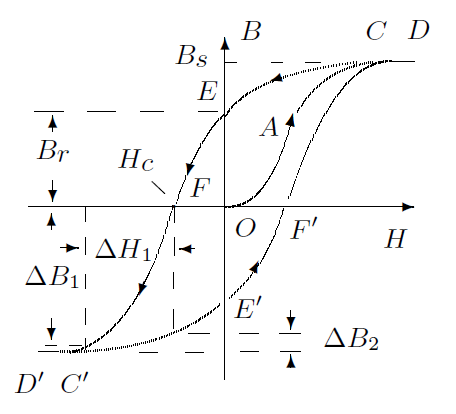
\includegraphics[width=41mm]{fig1.PNG}
\hfil
\caption{Петля гистерезиса ферромагнетика}
\label{figCurvesFF}
\end{floatingfigure}

Магнитная индукция \textbf{B} и напряжённость магнитного поля \textbf{H} в ферромагнетике неоднозначно связаны между собой: индукция зависит не только от напряжённости, но и от предыстории образца. В эксперименте будет исследоваться \textit{основная кривая намагничивания OACD} и \textit{предельная петля гистерезиса DEFD'E'F'D} (см. рис. 1).

С помощью баллистического гальванометра и амперметра будем косвенно измерять зависимость индукции магнитного поля от его напряжённости. \\
Напряжённость магнитного поля \textit{H} в тороиде зависит от тока, текущего в намагничивающей обмотке:
\begin{equation}
    H = \frac{N_{T_0}}{\pi D}I,
\end{equation}
где $D$ - средний диаметр тора, $N_{T_0}$ - количество витков.

Изменение поля приводит к изменению потока магнитной индукции Ф в сердечнике, в измерительной обмотке возникает ЭДС индукции, через гальванометр, в свою очередь, протекает импульс тока, изменяется положение рамки и, следовательно, зайчика. Окончательно (определив также баллистическую постоянную гальванометра, проведя измерения с соленоидом) для изменения магнитной индукции в сердечнике тороида получаем:
\begin{equation}
    \triangle B = \mu_0 (\frac{d_C}{d_T})^2 \frac{R}{R_1} \frac{N_{C_0}}{N_{T_1}} \frac{N_{C_1}}{l_C} \triangle I_1 \frac{\triangle x}{\triangle x_1},
\end{equation}
где $R$ - полное сопротивление измерительной цепи тороида, $d_C, d_T$ - диаметр поперечного сечения соленоида и тороида соответственно, $N_{C_0}$  - число витков пустотелого соленоида, $N_{C_1}$ - число витков короткой измерительной катушки $l_C$ - длина соленоида, $\triangle x_1$ - отклонение зайчика при работе с соленоидом, $\triangle x$ - отклонение зайчика в эксперименте.

\section{Экспериментальная установка}

\begin{figure}[h]
    \centering
    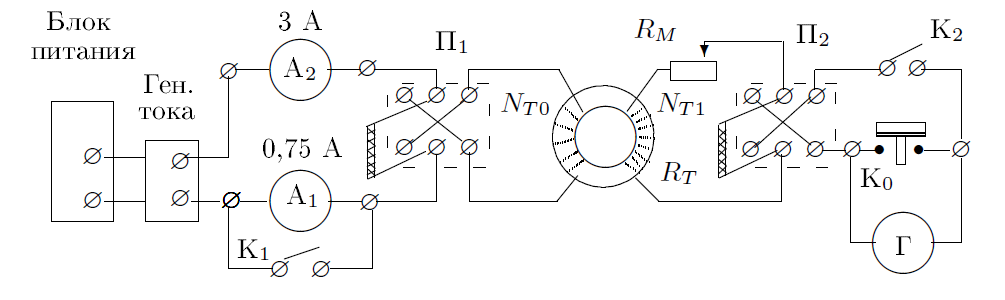
\includegraphics[width=10cm]{fig2.PNG}
    \caption{Схема установки для исследования петли гистерезиса}
    \label{fig:vac}
\end{figure}

\begin{figure}[h]
    \centering
    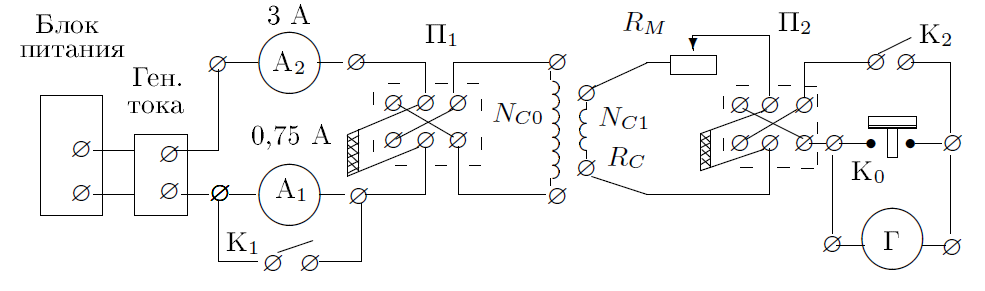
\includegraphics[width=10cm]{fig3.PNG}
    \caption{Схема установки для калибровки гальванометра}
    \label{fig:vac1}
\end{figure}

После снятия петли гистерезиса необходимо размагнитить сердечник, подключив его к цепи переменного тока, постепенно снижая его амплитуду. Только затем следует приступать к снятию основной кривой намагничивания.

\section{Ход работы}

\begin{enumerate}
    \item Подготовив к работе экспериментальную установку, снимем зависимость величины скачка $\triangle x$ от величины силы тока в цепи $I$. Пройдём по всей петле гистерезиса, результаты занесём в таблицу 1.

    \begin{center}
\begin{tabular}{|c|c|c|c|c|c|}\hline
$I\text{, mA}$&$\Delta I\text{, mA}$&$\Delta x\text{, у.ед}$&$I\text{, mA}$&$\Delta I\text{, mA}$&$\Delta x\text{, у.ед}$\\\hline
$1462$&$3$&$0$&$-1460$&$3$&$0$\\\hline
$515$&$1$&$-130$&$-515$&$1$&$137$\\\hline
$250.2$&$0.5$&$-112$&$-249.9$&$0.5$&$111$\\\hline
$157.0$&$0.3$&$-69$&$-156.9$&$0.3$&$88$\\\hline
$94.69$&$0.19$&$-59$&$-94.66$&$0.19$&$58$\\\hline
$66.50$&$0.13$&$-34$&$-66.51$&$0.13$&$34$\\\hline
$55.81$&$0.11$&$-18$&$-55.82$&$0.11$&$16$\\\hline
$44.47$&$0.09$&$-17$&$-44.47$&$0.09$&$16$\\\hline
$39.15$&$0.08$&$-7$&$-39.19$&$0.08$&$11$\\\hline
$28.09$&$0.06$&$-16$&$-28.10$&$0.06$&$16$\\\hline
$15.36$&$0.03$&$-21$&$-15.37$&$0.03$&$20$\\\hline
$0.11$&$0.01$&$-37$&$-0.14$&$0.01$&$37$\\\hline
$-15.38$&$0.03$&$-55$&$15.38$&$0.03$&$57$\\\hline
$-28.11$&$0.06$&$-68$&$28.11$&$0.06$&$70$\\\hline
$-39.12$&$0.08$&$-162$&$39.15$&$0.08$&$170$\\\hline
$-44.45$&$0.09$&$-114$&$44.46$&$0.09$&$122$\\\hline
$-55.81$&$0.11$&$-190$&$55.81$&$0.11$&$206$\\\hline
$-66.45$&$0.13$&$-96$&$66.50$&$0.13$&$100$\\\hline
$-94.56$&$0.19$&$-174$&$94.63$&$0.19$&$183$\\\hline
$-156.8$&$0.3$&$-172$&$156.8$&$0.3$&$187$\\\hline
$-249.9$&$0.5$&$-118$&$249.8$&$0.5$&$127$\\\hline
$-514$&$1$&$-147$&$514$&$1$&$161$\\\hline
$-1458$&$3$&$-130$&$1458$&$3$&$144$\\\hline
\end{tabular}\\~\\
$\Delta (\Delta x)=3\,\text{у.ед}$
\end{center}


Погрешность $I$ взята как $0.2\%I$, опираясь на даташит миллиамперметра.


\item
Для калибровки соберем установку на рис.5, уменьшим $R_\text{М}$ на $R_\text{С}$ и измерим отклонение гальванометра при изменении тока на $I_{max}$, разомкнув П1.
Получаются отклонения:
\begin{center}
\begin{tabular}{|c|c|c|c|c|c|}\hline
$\Delta x_1,\,\text{у.ед}$&$80$&$81$&$80$&$80$&$81$\\\hline
\end{tabular}\\~\\
$\Delta (\Delta x_1) = 0.5\,\text{у.ед}$,
\end{center}
Что в среднем дает $\Delta x_1=80.4\pm0.7\text{уд.ед.}$ (тут погрешность как корень суммы квадратов статистической и приборной погрешности).

\newpage
\item
Измерим кривую намагничивания, размагнитив тороид в установке ЛАТР, после чего повторим 5 пункт, меняя ток от $0$ до $I_{max}$:

\begin{center}
\begin{tabular}{|c|c|c|}\hline
$I\text{, mA}$&$\Delta I\text{, mA}$&$\Delta x\text{, у.ед}$\\\hline
$0$&$0$&$0$\\\hline
$15.38$&$0.03$&$23$\\\hline
$28.11$&$0.06$&$43$\\\hline
$39.14$&$0.08$&$102$\\\hline
$44.45$&$0.09$&$50$\\\hline
$55.80$&$0.11$&$94$\\\hline
$66.47$&$0.13$&$58$\\\hline
$94.62$&$0.19$&$128$\\\hline
$156.8$&$0.3$&$157$\\\hline
$249.8$&$0.5$&$126$\\\hline
$514$&$1$&$168$\\\hline
$1457$&$3$&$150$\\\hline
\end{tabular}\\~\\
$\Delta (\Delta x)=3\,\text{у.ед}$
\end{center}

\item
Запишем данные установки:\\
$N_\text{Т0}=1750$, $N_\text{Т1}=300$, $R_\text{С}=60\,\text{Ом}$, $l_\text{С}=80\,\text{см}$, $d_\text{С}=7\,\text{cм}$, $N_\text{C1}=435$, $N_\text{C0}=825$, $D=10\,\text{см}$, $d_\text{Т}=1\,\text{см}$.
\subsection*{обработка-1-3}
Используя формулы пересчета, найдем $H$ и $\Delta B$.
Проверим суммы $\Delta x$ на подьеме и спуске по петле. Они равны с точностью до $6\%$ ($2071\,\text{у.ед}$ и $1946\,\text{у.ед}$).
$$H=\frac{N_{T0}}{\pi D}I$$
$$\Delta B = \mu_0 \left(\frac{d_c}{d_T}\right)^2\frac{N_{C0}}{N_{T1}}\frac{N_{C1}}{l_C}\Delta I_1 \frac{\Delta x}{\Delta x_1}$$

Относительная погрешность $H$ равна относительной погрешности $I$, поскольку $D$ нам дано без погрешности.\\
По аналогичным причинам относительная погрешность $\Delta B$ равна сумме относительных погрешностей $\Delta I$, $\Delta x_1$ и $\Delta x$.

\newpage

Пересчет петли:
\begin{center}
\begin{tabular}{|c|c|c|c|c|c|c|c|}\hline
$H\text{, А/м}$&$\Delta H\text{, А/м}$&$\Delta B\text{, Тл}$&$\Delta (\Delta B)\text{, Тл}$&$H\text{, А/м}$&$\Delta H\text{, А/м}$&$\Delta B\text{, Тл}$&$\Delta (\Delta B)\text{, Тл}$\\\hline
$8143$&$16$&$0$&$0$&$-8133$&$16$&$0$&$0$\\\hline
$2867$&$6$&$-0.220$&$0.006$&$-2867$&$6$&$0.232$&$0.006$\\\hline
$1393$&$3$&$-0.189$&$0.005$&$-1392$&$3$&$0.188$&$0.005$\\\hline
$874.7$&$1.7$&$-0.116$&$0.005$&$-873.9$&$1.7$&$0.149$&$0.005$\\\hline
$527.5$&$1.1$&$-0.099$&$0.004$&$-527.2$&$1.1$&$0.098$&$0.004$\\\hline
$370.4$&$0.7$&$-0.057$&$0.004$&$-370.4$&$0.7$&$0.058$&$0.004$\\\hline
$310.9$&$0.6$&$-0.030$&$0.004$&$-310.9$&$0.6$&$0.027$&$0.004$\\\hline
$247.7$&$0.5$&$-0.028$&$0.004$&$-247.7$&$0.5$&$0.027$&$0.004$\\\hline
$218.1$&$0.4$&$-0.011$&$0.004$&$-218.3$&$0.4$&$0.019$&$0.004$\\\hline
$156.5$&$0.3$&$-0.027$&$0.004$&$-156.5$&$0.3$&$0.027$&$0.004$\\\hline
$85.56$&$0.17$&$-0.035$&$0.004$&$-85.61$&$0.17$&$0.034$&$0.004$\\\hline
$0.61$&$0.01$&$-0.062$&$0.004$&$-0.78$&$0.01$&$0.063$&$0.004$\\\hline
$-85.67$&$0.17$&$-0.093$&$0.004$&$85.67$&$0.17$&$0.097$&$0.004$\\\hline
$-156.5$&$0.3$&$-0.115$&$0.005$&$156.6$&$0.3$&$0.119$&$0.005$\\\hline
$-217.9$&$0.4$&$-0.274$&$0.006$&$218.1$&$0.4$&$0.288$&$0.006$\\\hline
$-247.6$&$0.5$&$-0.193$&$0.005$&$247.7$&$0.5$&$0.207$&$0.006$\\\hline
$-310.8$&$0.6$&$-0.321$&$0.007$&$310.9$&$0.6$&$0.349$&$0.007$\\\hline
$-370.1$&$0.7$&$-0.162$&$0.005$&$370.4$&$0.7$&$0.169$&$0.005$\\\hline
$-526.7$&$1.1$&$-0.294$&$0.007$&$527.1$&$1.1$&$0.310$&$0.007$\\\hline
$-873.7$&$1.7$&$-0.291$&$0.007$&$873.6$&$1.7$&$0.317$&$0.007$\\\hline
$-1392$&$3$&$-0.199$&$0.006$&$1391$&$3$&$0.215$&$0.006$\\\hline
$-2862$&$6$&$-0.249$&$0.006$&$2862$&$6$&$0.273$&$0.006$\\\hline
$-8125$&$16$&$-0.220$&$0.006$&$8122$&$16$&$0.244$&$0.006$\\\hline
\end{tabular}\\~\\
\end{center}

Пересчет кривой намагничивания:
\begin{center}
\begin{tabular}{|c|c|c|c|}\hline
$H\text{, А/м}$&$\Delta H\text{, А/м}$&$\Delta B\text{, Тл}$&$\Delta (\Delta B)\text{, Тл}$\\\hline
$0$&$0$&$0$&$0$\\\hline
$85.67$&$0.17$&$0.039$&$0.004$\\\hline
$156.6$&$0.3$&$0.073$&$0.004$\\\hline
$218.0$&$0.4$&$0.173$&$0.005$\\\hline
$247.6$&$0.5$&$0.085$&$0.004$\\\hline
$310.8$&$0.6$&$0.159$&$0.005$\\\hline
$370.3$&$0.7$&$0.098$&$0.004$\\\hline
$527.1$&$1.1$&$0.217$&$0.006$\\\hline
$873.4$&$1.7$&$0.266$&$0.006$\\\hline
$1391$&$3$&$0.214$&$0.006$\\\hline
$2862$&$6$&$0.285$&$0.006$\\\hline
$8117$&$16$&$0.254$&$0.006$\\\hline
\end{tabular}\\~\\
\end{center}
Теперь посчитаем $B$ через $\Delta B$ обычным суммированием:
$$B_{i+1} = B_{i} + \Delta B_{i+1}, \Delta_\text{п} B_{i+1} = \Delta_\text{п} B_{i} + \Delta_\text{п} \Delta B_{i+1},$$
где $\Delta_\text{п}$ -- погрешность (чтобы не путать $\Delta_\text{п} B$ и $\Delta B$).
При этом за $B_0$ возьмем половину средней (по двум направлениям) высоты $B$ петли. Она равна:
$$B_0 = -0.5 \frac{3.29 + 3.51}{2}\,\text{Тл} = -1.70\,\text{Тл}.$$

\newpage
Пересчет $B$ петли:
\begin{center}
\begin{tabular}{|c|c|c|c|c|c|c|c|}\hline
$H\text{, А/м}$&$\Delta H\text{, А/м}$&$B\text{, Тл}$&$\Delta B\text{, Тл}$&$H\text{, А/м}$&$\Delta H\text{, А/м}$&$B\text{, Тл}$&$\Delta B\text{, Тл}$\\\hline
$8143$&$16$&$1.60$&$0.11$&$-8133$&$16$&$-1.7$&$0$\\\hline
$2867$&$6$&$1.4$&$0.1$&$-2867$&$6$&$-1.467$&$0.006$\\\hline
$1393$&$3$&$1.2$&$0.1$&$-1392$&$3$&$-1.279$&$0.011$\\\hline
$874.7$&$1.7$&$1.07$&$0.09$&$-873.9$&$1.7$&$-1.130$&$0.016$\\\hline
$527.5$&$1.1$&$0.97$&$0.09$&$-527.2$&$1.1$&$-1.03$&$0.02$\\\hline
$370.4$&$0.7$&$0.91$&$0.09$&$-370.4$&$0.7$&$-0.97$&$0.02$\\\hline
$310.9$&$0.6$&$0.88$&$0.08$&$-310.9$&$0.6$&$-0.94$&$0.03$\\\hline
$247.7$&$0.5$&$0.85$&$0.08$&$-247.7$&$0.5$&$-0.92$&$0.03$\\\hline
$218.1$&$0.4$&$0.84$&$0.07$&$-218.3$&$0.4$&$-0.90$&$0.04$\\\hline
$156.5$&$0.3$&$0.81$&$0.07$&$-156.5$&$0.3$&$-0.87$&$0.04$\\\hline
$85.56$&$0.17$&$0.78$&$0.07$&$-85.61$&$0.17$&$-0.84$&$0.04$\\\hline
$0.61$&$0.01$&$0.72$&$0.06$&$-0.78$&$0.01$&$-0.77$&$0.05$\\\hline
$-85.67$&$0.17$&$0.62$&$0.06$&$85.67$&$0.17$&$-0.68$&$0.05$\\\hline
$-156.5$&$0.3$&$0.51$&$0.05$&$156.6$&$0.3$&$-0.56$&$0.06$\\\hline
$-217.9$&$0.4$&$0.23$&$0.05$&$218.1$&$0.4$&$-0.27$&$0.06$\\\hline
$-247.6$&$0.5$&$0.04$&$0.04$&$247.7$&$0.5$&$-0.06$&$0.07$\\\hline
$-310.8$&$0.6$&$-0.28$&$0.04$&$310.9$&$0.6$&$0.28$&$0.08$\\\hline
$-370.1$&$0.7$&$-0.44$&$0.03$&$370.4$&$0.7$&$0.45$&$0.08$\\\hline
$-526.7$&$1.1$&$-0.73$&$0.02$&$527.1$&$1.1$&$0.76$&$0.09$\\\hline
$-873.7$&$1.7$&$-1.030$&$0.017$&$873.6$&$1.7$&$1.08$&$0.09$\\\hline
$-1392$&$3$&$-1.230$&$0.012$&$1391$&$3$&$1.3$&$0.1$\\\hline
$-2862$&$6$&$-1.479$&$0.006$&$2862$&$6$&$1.57$&$0.11$\\\hline
$-8125$&$16$&$-1.7$&$0$&$8122$&$16$&$1.81$&$0.11$\\\hline
\end{tabular}\\~\\
\end{center}


Пересчет $B$ кривой намагничивания:
\begin{center}
\begin{tabular}{|c|c|c|c|}\hline
$H\text{, А/м}$&$\Delta H\text{, А/м}$&$B\text{, Тл}$&$\Delta B\text{, Тл}$\\\hline
$0$&$0$&$0$&$0$\\\hline
$85.67$&$0.17$&$0.039$&$0.004$\\\hline
$156.6$&$0.3$&$0.073$&$0.008$\\\hline
$218.0$&$0.4$&$0.173$&$0.013$\\\hline
$247.6$&$0.5$&$0.085$&$0.018$\\\hline
$310.8$&$0.6$&$0.16$&$0.02$\\\hline
$370.3$&$0.7$&$0.10$&$0.03$\\\hline
$527.1$&$1.1$&$0.22$&$0.03$\\\hline
$873.4$&$1.7$&$0.27$&$0.04$\\\hline
$1391$&$3$&$0.21$&$0.04$\\\hline
$2862$&$6$&$0.28$&$0.05$\\\hline
$8117$&$16$&$0.25$&$0.06$\\\hline
\end{tabular}\\~\\
\end{center}

\begin{center}
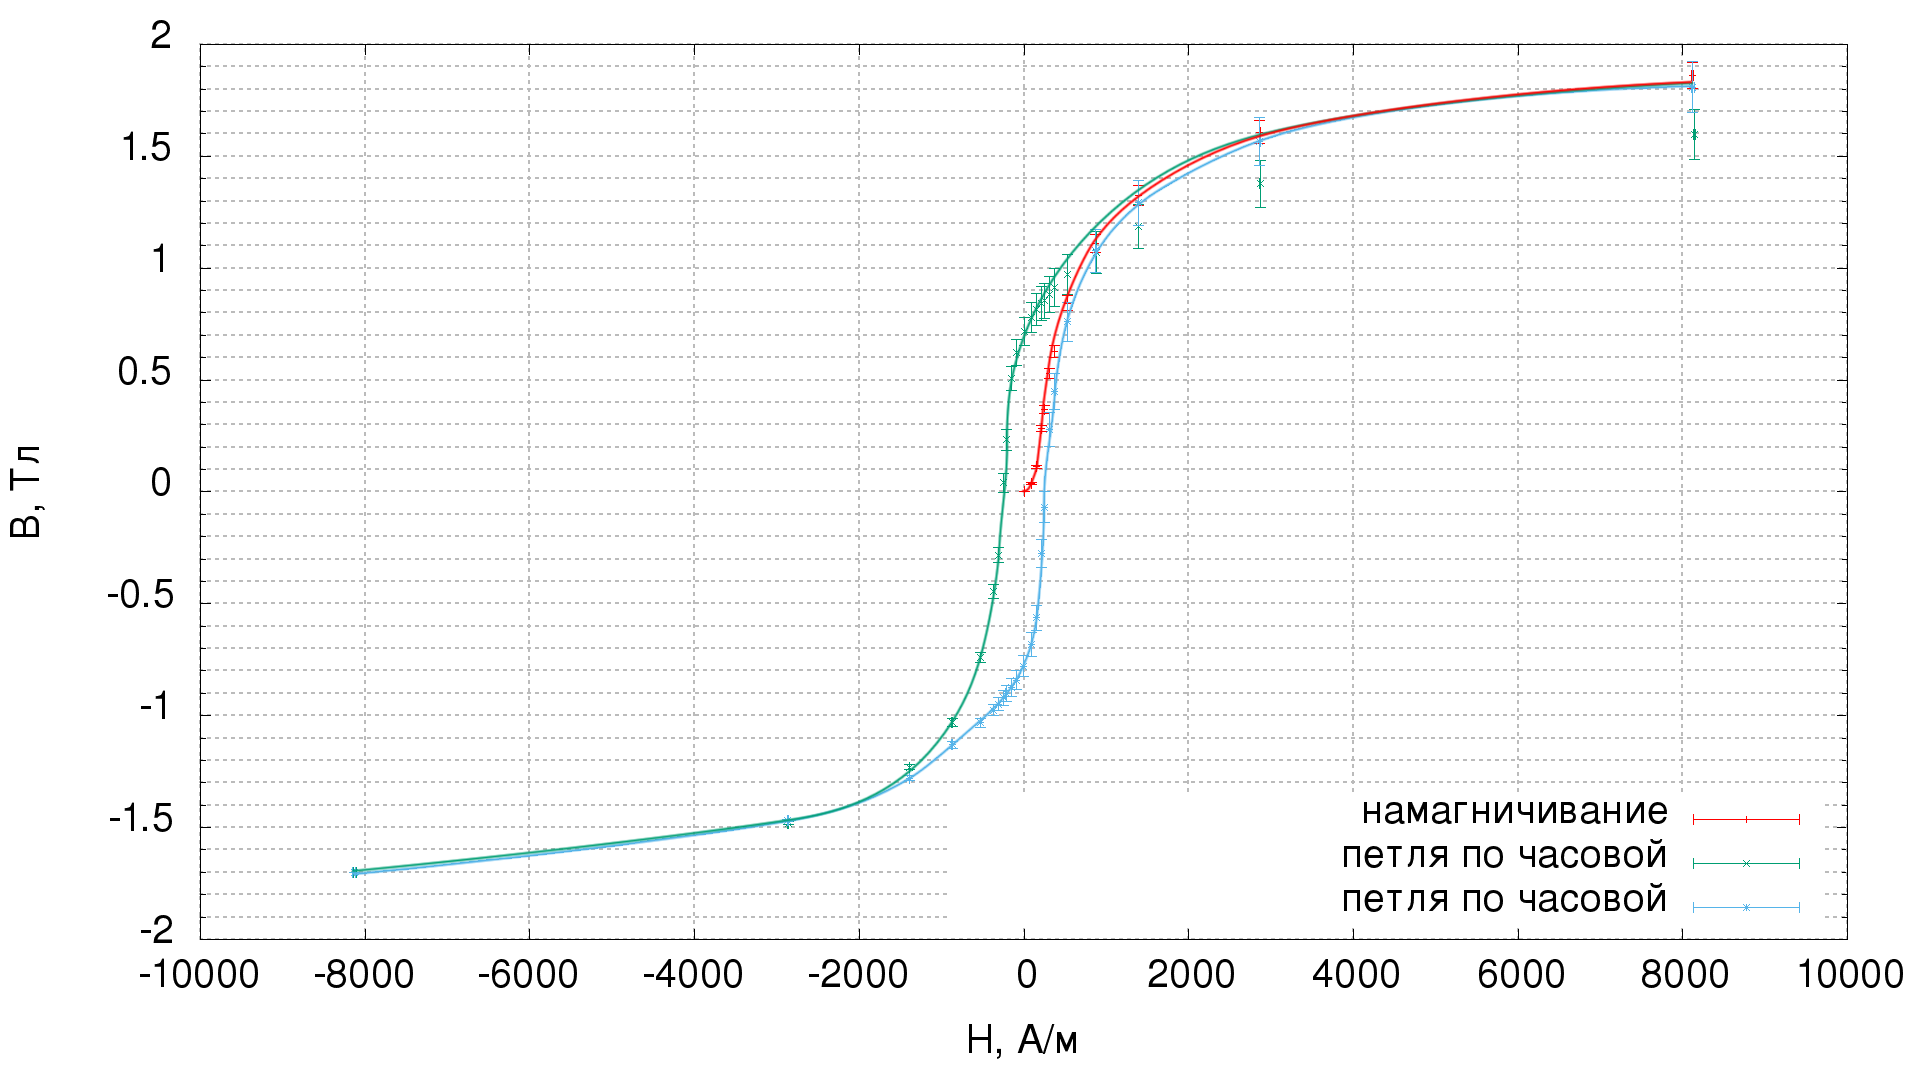
\includegraphics[width=\textwidth]{5_big.png}
\end{center}
\begin{center}
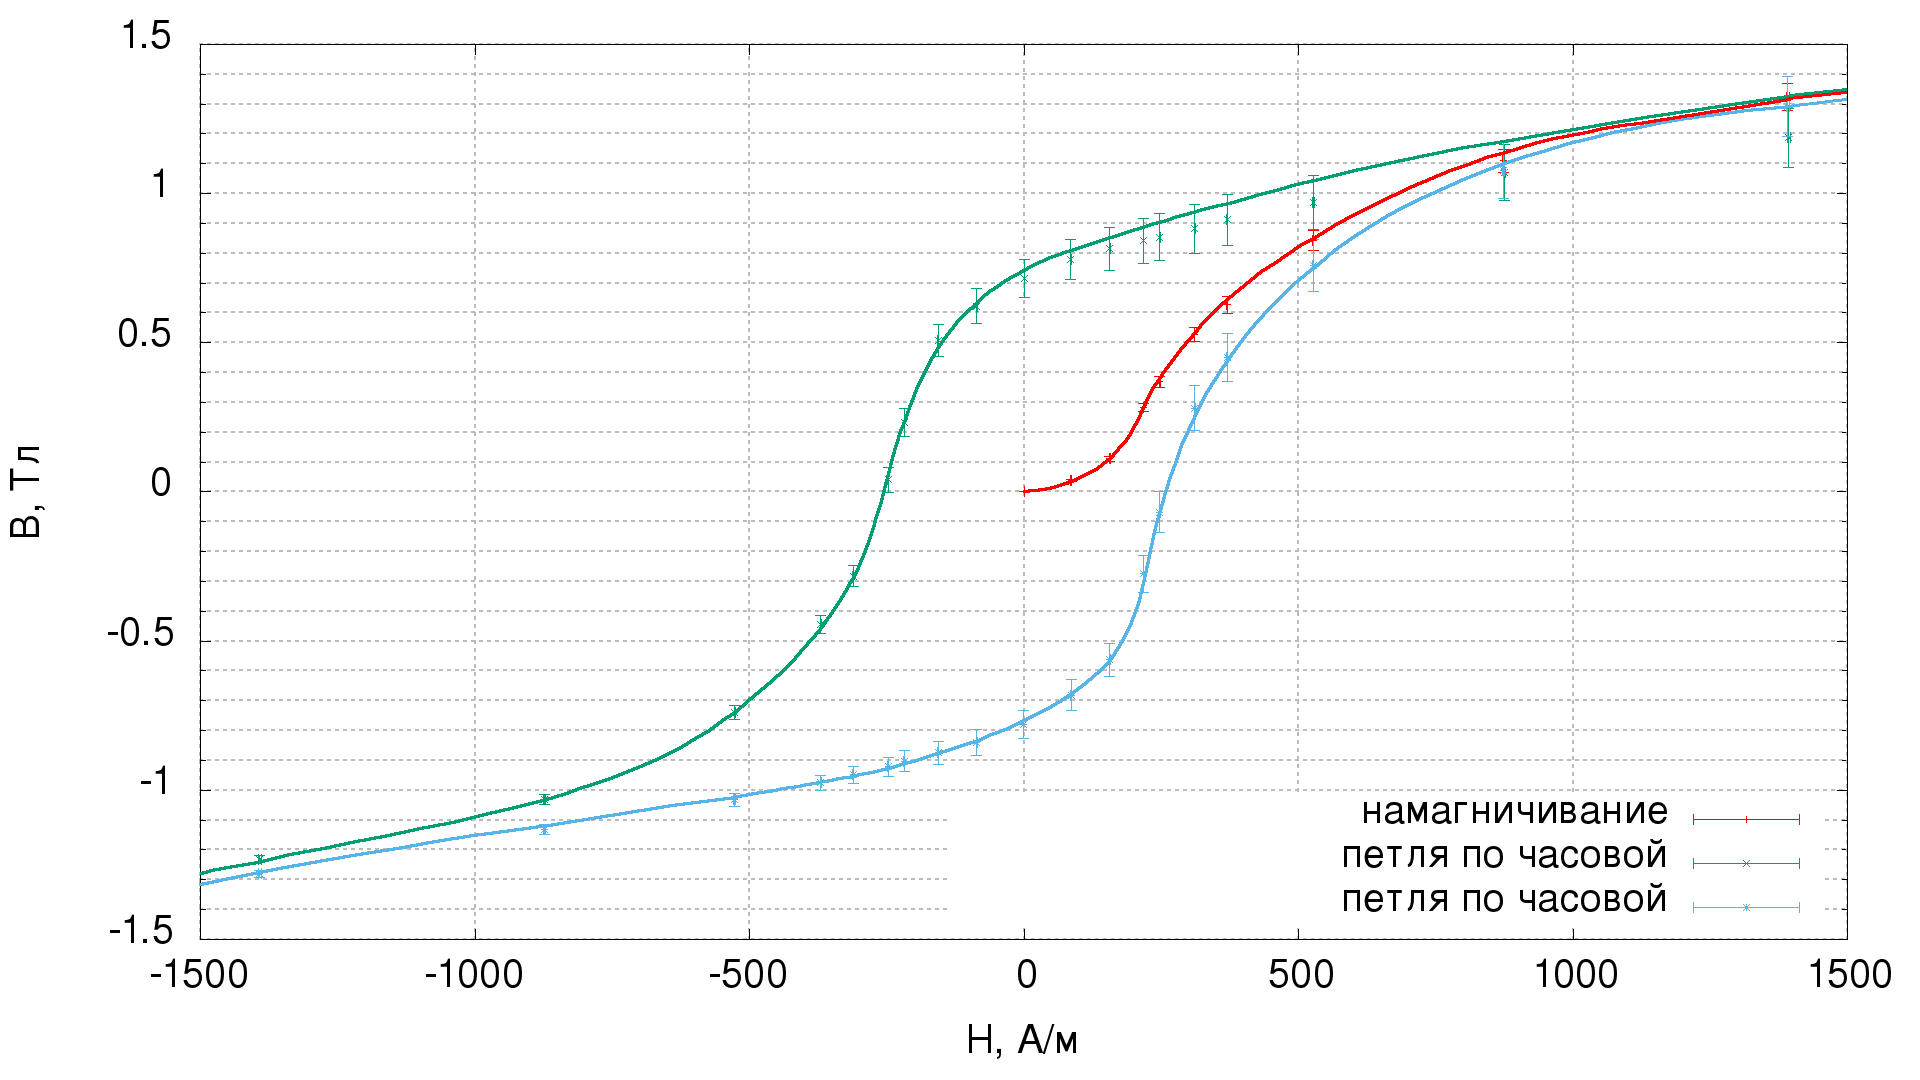
\includegraphics[width=\textwidth]{5_small.png}
\end{center}

Из графиков:\\
Коэрцитивная сила $H_{c}=500*\frac{143\pm2}{275\pm2}\,\text{А}/\text{м} = 260\pm6\,\text{А}/\text{м}.$ (погрешность из толщины линии)\\
Индукция насыщения $B_s = (1.70\pm0.16)\,\text{Тл}$ (погрешность как корень суммы квадратов погрешности $\Delta B$ ($0.11\,\text{Тл}$) и половины разности между $B_s$ для разных направлений ($0.11\,\text{Тл}$)).

Для того, чтобы посчитать $\mu_\text{диф}$ я распечатал график, провел касательную и отсканировал график. Используя пропорции по пикселям я нашел :
$$\frac{dB}{dH} = \frac{1391-403\pm8}{2323-1856\pm8}\frac{3256-458\pm8}{1868-357\pm8}\frac{3\,\text{Тл}}{3000\,\text{А}/\text{м}} = (3.91\pm0.13) \frac{\text{мм}\,\text{Тл}}{\text{А}}.$$
$$\mu_\text{диф} = \frac{dB}{\mu_0dH} = 3100\pm100$$
График для демонстрации того, что я сделал, его почти полная копия выше.
\begin{center}
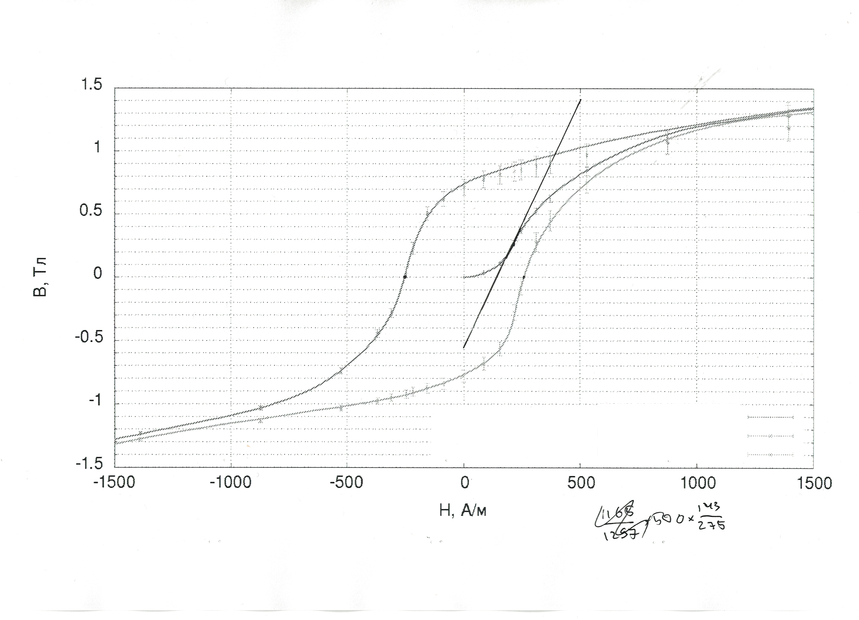
\includegraphics[width=0.99\textwidth]{6_res.png}
\end{center}

\end{enumerate}

\begin{center}
\begin{tabular}{|c|c|c|}
\hline
&Эксперимент&таблица\\\hline
$\mu_\text{диф}$&$3100\pm100$&$5000$\\\hline
$B_s,\,\text{Тл}$&$1.70\pm0.16$&$2.15$\\\hline
$H_{c}\,\text{А}/\text{м}$&$260\pm6$&$80$\\\hline
\end{tabular}
\end{center}
\section{Вывод}
Мы промерили петлю и кривую намагничивания у магнитного гистерезиса с помощью статического метода и получили значения индукции насыщения и дифференциальной магнитной проницаемости с отклонением от табличного значения менее чем на $30\%$ и $60\%$ соответственно, а также выяснили коэрцитивную силу менее, чем в $4$ раза превышающей табличное значение. Полученные отклонения я могу объяснить уникальностью характеристик установки, из-за чего реальные параметры могут сильно отличаться от табличных.

%     \begin{table}[h]
%     \centering
%     \begin{center}
%     \caption{Зависимость $\triangle x$ от $I$ и соответствующие $H$ и $\triangle B$, петля гистерезиса}
%     \end{center}
%     \vspace{0.1cm}
%     \label{tab:my_label}
%     \begin{tabular}{ |p{1.2cm}||p{1cm}|p{1cm}|p{1cm}|p{1cm}|p{1cm}|p{1cm}|p{1cm}|p{1cm}|p{1cm}|p{1cm}|p{1cm}|p{1cm}| }
%  \hline
%     $I$, мA & 538 & 244 & 146.7 & 96.3 & 64.7 & 49.3 & 39.8 & 33.9 & 30.9 & 27.2 & 23.6 & 0.63 \\
% \hline
%     $\triangle x$, см & 6.9 & 6.8 & 4.95 & 3.7 & 2.9 & 1.7 & 1.13 & 0.7 & 0.4 & 0.5 & 0.5 & 4.1 \\
% \hline
%     $H$, А/м & 299.84 & 135.987 & 81.760 & 53.670 & 36.059 & 27.476 & 22.182 & 18.893 & 17.221 & 15.159 & 13.153 & 0.351\\
% \hline
%     $\triangle B$, Тл & 0.002 & 0.211 & 0.166 & 0.124 & 0.097 & 0.057 & 0.038 & 0.023 & 0.014 & 0.010 & 0.007 & 0.007\\
% \hline
% \hline

%     $I$, мА & 0.00 & 0.6 & 23.7 & 27.3 & 31.1 & 34.1 & 40.2 & 49.6 & 64.8 & 96.3 & 146.9 & 244.2 \\
% \hline
%     $\triangle x$, см & 0.1 & 0.1 & 6.9 & 1.6 & 2.3 & 2.45 & 7.5 & 11.8 & 11.3 & 12.2 & 9.3 & 8.9 \\
% \hline
%     $H$, А/м & 0.00 & -0.33 & -13.21 & -15.22 & -17.33 & -19.01 & -22.40 & -27.64 & -36.12 & -53.67 & -81.87 & -136.1 \\
% \hline
%     $\triangle B$, Тл & 0.003 & 0.007 & 0.231 & 0.054 & 0.077 & 0.082 & 0.251 & 0.395 & 0.379 & 0.409 & 0.312 & 0.298 \\

% \hline
% \hline

%     $I$, мА & 537 & 244.1 & 146.8 & 96.3 & 64.8 & 49.3 & 39.8 & 33.9 & 31 & 27.2 & 23.5 & 0.62 \\
% \hline
%     $\triangle x$, см & 17.7 & 11 & 7.85 & 5.8 & 4.6 & 2.6 & 1.8 & 1.15 & 0.6 & 0.8 & 0.8 & 6.4 \\
% \hline
%     $H$, А/м & -299.3 & -136.0 & -81.82 & -53.67 & -36.11 & -27.48 & -22.18 & -18.89 & -17.28 & -15.16 & -13.10 & -0.35\\
% \hline
%     $\triangle B$, Тл & 0.570 & 0.369 & 0.263 & 0.194 & 0.154 & 0.087 & 0.060 & 0.039 & 0.020 & 0.027 & 0.027 & 0.214\\
% \hline
% \hline

%     $I$, мА & 0.00 & 0.6 & 27.3 & 31.1 & 34.1 & 40.1 & 49.6 & 64.9 & 96.4 & 146.8 & 244.1 \\
% \hline
%     $\triangle x$, см & 0.2 & 0.2 & 2.5 & 3.6 & 3.9 & 6.9 & 9.2 & 10.6 & 10.8 & 8.0 & 7.7 & 7.6 \\
% \hline
%     $H$, А/м & 0.000 & 0.351 & 15.215 & 17.333 & 19.005 & 22.349 & 27.643 & 36.170 & 53.726 & 81.815 & 136.043 & 299.841 \\
% \hline
%     $\triangle B$, Тл & 0.007 & 0.005 & 0.084 & 0.121 & 0.131 & 0.231 & 0.308 & 0.355 & 0.362 & 0.268 & 0.258 & 0.255 \\
% \hline
% \hline
%     \end{tabular}
% \end{table}

% \item Отсоединим цепь от тороида, подсоединим её к пустотелому соленоиду. Откалибруем гальванометр. Получившиеся необходимые значения:

% \begin{center}
%     $I_{max}  = 1.473 A$ \hspace{1cm} $\triangle x_{1} = 7.9$ см
% \end{center}

% \item Размагнитим тороид с помощью источника переменного тока и трансформатора. Снимем начальную кривую намагничивания, результаты занесём в таблицу 2.

%    \begin{table}[h]
%     \centering
%     \begin{center}
%     \caption{Зависимость $\triangle x$ от $I$ и соответствующие $H$ и $\triangle B$, начальная кривая намагничивания}
%     \end{center}
%     \vspace{0.1cm}
%     \label{tab:my_label}
%     \begin{tabular}{ |p{1.2cm}||p{1cm}|p{1cm}|p{1cm}|p{1cm}|p{1cm}|p{1cm}|p{1cm}|p{1cm}|p{1cm}|p{1cm}|p{1cm}|p{1cm}| }
%  \hline
%     $I$, мА & 0.6 & 27.3 & 31.1 & 34.1 & 40.1 & 49.6 & 64.9 & 96.4 & 146.8 & 244.1 & 537 \\
% \hline
%     $\triangle x$, см & 0.1 & 5.8 & 1.8 & 2.5 & 2.3 & 5.4 & 8.4 & 11.1 & 15.8 & 15.5 & 18.1 & 18.1 \\
% \hline
%     $H$, А/м & 0.368 & 13.209 & 15.271 & 17.389 & 19.061 & 22.404 & 27.699 & 36.170 & 53.726 & 81.927 & 136.154 & 299.283\\
% \hline
%     $\triangle B$, Тл & 0.001 & 0.100 & 0.031 & 0.043 & 0.039 & 0.093 & 0.144 & 0.191 & 0.266 & 0.271 & 0.294 & 0.311\\
% \hline
% \hline

%     \end{tabular}
% \end{table}

% \item В координатах $B(H)$ построим на одном графике петлю гистерезиса и начальную кривую намагничивания (рисунок 4).

% \begin{figure}[h]
%     \centeringimport numpy as np
%     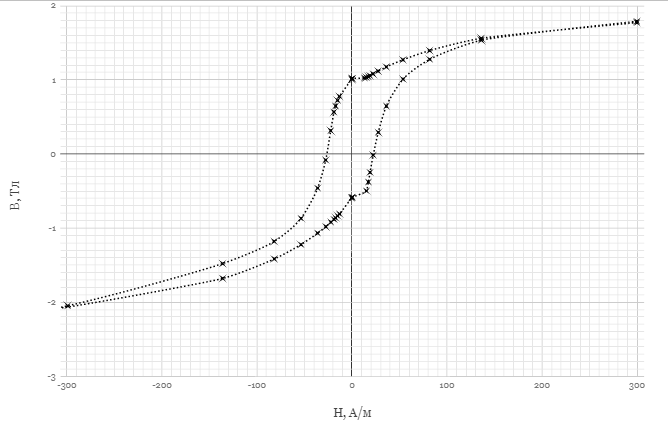
\includegraphics[width=\textwidth]{graph1.PNG}
%     \caption{Петля гистерезиса и начальная кривая намагничивания для исследуемого образца}
%     \label{fig:vac}
% \end{figure}

% По графику определим следующие величины и оценим их погрешности:
% \begin{itemize}
%     \item коэрцитивная сила $H_c$ - значение напряжённости магнитного поля, необходимое для полного размагничивания ферромагнитного вещества равна длине отрезка, высекаемого петлёй гистерезиса на горизонтальной оси. $H_c = 55 \pm 3.3$ А/м.
%     \item индукция насыщения $B_s$ -  максимально достижимое значение внутренней индукции магнитного материала при данной температуре. $B_s = 1.95 \pm 0.3$ Тл.
%     \item максимальная дифференциальная магнитная проницаемость $\mu_d = \frac{1}{\mu_0}\frac{dB}{dH}$ - характеризующий связь между магнитной индукцией B и напряжённостью магнитного поля H в веществе. $\mu_d = 9715 \pm 270$
% \end{itemize}

% Итоговые результаты сведём в таблицу. Теоретические значения возьмём из справочника в пособии к лабораторным работам для технической стали.

%    \begin{table}[h]
%     \centering
%     \begin{center}
%     \caption{Соответствие теоретических и экспериментальных результатов}
%     \end{center}
%     \vspace{0.1cm}
%     \label{tab:my_label}
%     \begin{tabular}{ |p{2cm}||p{3cm}|p{3cm}| }
%  \hline
%      & Эксперимент & Справочник\\
% \hline
% \hline
%      $H_c$, А/м & $55 \pm 3.3$ & 80  \\
% \hline
%     $B_s$, Тл & $1.95 \pm 0.3$ & 2.15 \\
% \hline
% \hline
%     $\mu_0$ & $9715 \pm 270$ & 5000 \\

%     \end{tabular}
% \end{table}

% \section{Вывод}

% В ходе работы были исследованы петля гистерезиса магнитомягкого материала, его начальная кривая намагничивания, с хорошей точностью экспериментально определены некоторые магнитные свойства. По кривой гистерезиса видно, что материал является магнитомягким, так как площадь петли мала. Также она симметрична и в целом соответствует теоретическим изображениям подобных кривых. Различие справочных и экспериментальных данных может объясняться тем, что, скорее всего, образец изготовлен не из чисто технического железа, а из сплава его с другим металлом.

\end{document}
